% Generated by TikzMakie.jl. Requires \usepackage{tikz} (and graphicx if images are used).
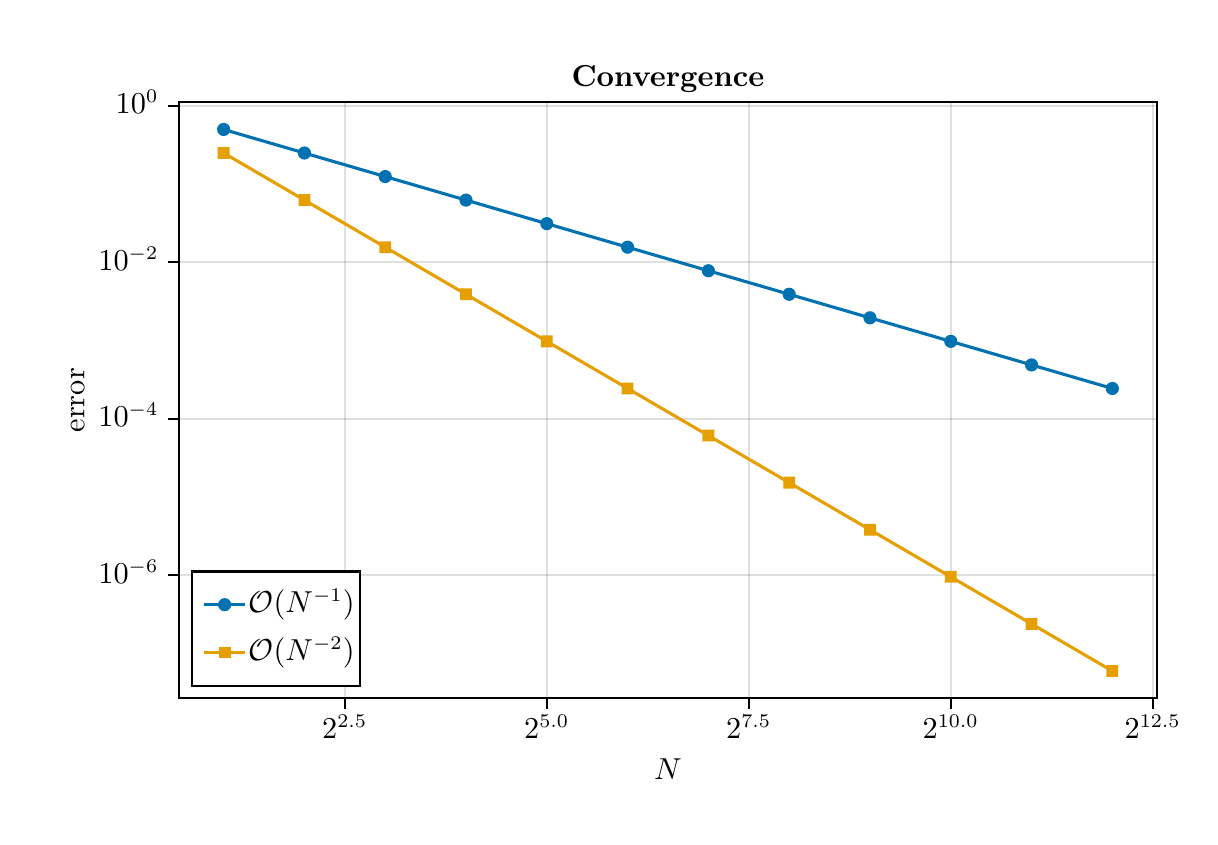
\begin{tikzpicture}[x=0.75pt, y=0.75pt, mknode/.style={inner sep=0pt, outer sep=0pt, execute at begin node={\vphantom{(}}, font=\fontsize{10.5}{12.6}\selectfont}, mkimg/.style={inner sep=0pt, outer sep=0pt}]
\definecolor{mkc1}{RGB}{0,114,178}
\definecolor{mkc2}{RGB}{230,159,0}
\path[use as bounding box] (0,0) rectangle (560,380);
\path[fill=white] (73,57) -- (544,57) -- (544,344) -- (73,344) -- cycle;
\draw[draw=black, line width=0.75pt, draw opacity=0.12]
  (152.8,57) -- (152.8,344)
  (250.11,57) -- (250.11,344)
  (347.43,57) -- (347.43,344)
  (444.74,57) -- (444.74,344)
  (542.05,57) -- (542.05,344);
\draw[draw=black, line width=0.75pt, draw opacity=0.12]
  (73,116.2) -- (544,116.2)
  (73,191.56) -- (544,191.56)
  (73,266.93) -- (544,266.93)
  (73,342.3) -- (544,342.3);
\node[mknode, anchor=north] at (308.5,28.6) {$N$};
\node[mknode, anchor=north] at (152.8,49) {$2^{2.5}$};
\node[mknode, anchor=north] at (250.11,49) {$2^{5.0}$};
\node[mknode, anchor=north] at (347.43,49) {$2^{7.5}$};
\node[mknode, anchor=north] at (444.74,49) {$2^{10.0}$};
\node[mknode, anchor=north] at (542.05,49) {$2^{12.5}$};
\node[mknode, anchor=south, rotate=90] at (30.97,200.5) {error};
\node[mknode, anchor=east] at (63,116.2) {$10^{-6}$};
\node[mknode, anchor=east] at (63,191.56) {$10^{-4}$};
\node[mknode, anchor=east] at (63,266.93) {$10^{-2}$};
\node[mknode, anchor=east] at (63,342.3) {$10^{0}$};
\node[mknode, anchor=south, font=\fontsize{10.5}{12.6}\selectfont\bfseries] at (308.5,348) {Convergence};
\begin{scope}
\clip (73,57) rectangle (544,344);
\draw[draw=mkc1, line width=1.12pt, miter limit=2]
  (94.41,330.95) -- (522.59,206.17);
\path[fill=mkc1] (97.58,330.95) -- (97.58,330.95) .. controls (97.58,332.71) and (96.16,334.13) .. (94.41,334.13) .. controls (92.66,334.13) and (91.24,332.71) .. (91.24,330.95) .. controls (91.24,329.2) and (92.66,327.78) .. (94.41,327.78) .. controls (96.16,327.78) and (97.58,329.2) .. (97.58,330.95) -- cycle (136.51,319.61) -- (136.51,319.61) .. controls (136.51,321.36) and (135.09,322.78) .. (133.33,322.78) .. controls (131.58,322.78) and (130.16,321.36) .. (130.16,319.61) .. controls (130.16,317.86) and (131.58,316.44) .. (133.33,316.44) .. controls (135.09,316.44) and (136.51,317.86) .. (136.51,319.61) -- cycle (175.43,308.27) -- (175.43,308.27) .. controls (175.43,310.02) and (174.01,311.44) .. (172.26,311.44) .. controls (170.51,311.44) and (169.09,310.02) .. (169.09,308.27) .. controls (169.09,306.51) and (170.51,305.09) .. (172.26,305.09) .. controls (174.01,305.09) and (175.43,306.51) .. (175.43,308.27) -- cycle (214.36,296.92) -- (214.36,296.92) .. controls (214.36,298.68) and (212.94,300.1) .. (211.19,300.1) .. controls (209.43,300.1) and (208.01,298.68) .. (208.01,296.92) .. controls (208.01,295.17) and (209.43,293.75) .. (211.19,293.75) .. controls (212.94,293.75) and (214.36,295.17) .. (214.36,296.92) -- cycle (253.28,285.58) -- (253.28,285.58) .. controls (253.28,287.33) and (251.86,288.75) .. (250.11,288.75) .. controls (248.36,288.75) and (246.94,287.33) .. (246.94,285.58) .. controls (246.94,283.83) and (248.36,282.41) .. (250.11,282.41) .. controls (251.86,282.41) and (253.28,283.83) .. (253.28,285.58) -- cycle (292.21,274.24) -- (292.21,274.24) .. controls (292.21,275.99) and (290.79,277.41) .. (289.04,277.41) .. controls (287.29,277.41) and (285.86,275.99) .. (285.86,274.24) .. controls (285.86,272.48) and (287.29,271.06) .. (289.04,271.06) .. controls (290.79,271.06) and (292.21,272.48) .. (292.21,274.24) -- cycle (331.14,262.89) -- (331.14,262.89) .. controls (331.14,264.64) and (329.71,266.06) .. (327.96,266.06) .. controls (326.21,266.06) and (324.79,264.64) .. (324.79,262.89) .. controls (324.79,261.14) and (326.21,259.72) .. (327.96,259.72) .. controls (329.71,259.72) and (331.14,261.14) .. (331.14,262.89) -- cycle (370.06,251.55) -- (370.06,251.55) .. controls (370.06,253.3) and (368.64,254.72) .. (366.89,254.72) .. controls (365.14,254.72) and (363.72,253.3) .. (363.72,251.55) .. controls (363.72,249.8) and (365.14,248.37) .. (366.89,248.37) .. controls (368.64,248.37) and (370.06,249.8) .. (370.06,251.55) -- cycle;
\path[fill=mkc1] (408.99,240.2) -- (408.99,240.2) .. controls (408.99,241.96) and (407.57,243.38) .. (405.81,243.38) .. controls (404.06,243.38) and (402.64,241.96) .. (402.64,240.2) .. controls (402.64,238.45) and (404.06,237.03) .. (405.81,237.03) .. controls (407.57,237.03) and (408.99,238.45) .. (408.99,240.2) -- cycle (447.91,228.86) -- (447.91,228.86) .. controls (447.91,230.61) and (446.49,232.03) .. (444.74,232.03) .. controls (442.99,232.03) and (441.57,230.61) .. (441.57,228.86) .. controls (441.57,227.11) and (442.99,225.69) .. (444.74,225.69) .. controls (446.49,225.69) and (447.91,227.11) .. (447.91,228.86) -- cycle (486.84,217.52) -- (486.84,217.52) .. controls (486.84,219.27) and (485.42,220.69) .. (483.67,220.69) .. controls (481.91,220.69) and (480.49,219.27) .. (480.49,217.52) .. controls (480.49,215.76) and (481.91,214.34) .. (483.67,214.34) .. controls (485.42,214.34) and (486.84,215.76) .. (486.84,217.52) -- cycle (525.76,206.17) -- (525.76,206.17) .. controls (525.76,207.92) and (524.34,209.34) .. (522.59,209.34) .. controls (520.84,209.34) and (519.42,207.92) .. (519.42,206.17) .. controls (519.42,204.42) and (520.84,203) .. (522.59,203) .. controls (524.34,203) and (525.76,204.42) .. (525.76,206.17) -- cycle;
\draw[draw=mkc2, line width=1.12pt, miter limit=2]
  (94.41,319.61) -- (522.59,70.05);
\path[fill=mkc2] (97.25,316.77) -- (97.25,322.45) -- (91.57,322.45) -- (91.57,316.77) -- cycle (136.18,294.08) -- (136.18,299.76) -- (130.49,299.76) -- (130.49,294.08) -- cycle (175.1,271.39) -- (175.1,277.08) -- (169.42,277.08) -- (169.42,271.39) -- cycle (214.03,248.71) -- (214.03,254.39) -- (208.34,254.39) -- (208.34,248.71) -- cycle (252.95,226.02) -- (252.95,231.7) -- (247.27,231.7) -- (247.27,226.02) -- cycle (291.88,203.33) -- (291.88,209.01) -- (286.2,209.01) -- (286.2,203.33) -- cycle (330.8,180.64) -- (330.8,186.33) -- (325.12,186.33) -- (325.12,180.64) -- cycle (369.73,157.95) -- (369.73,163.64) -- (364.05,163.64) -- (364.05,157.95) -- cycle;
\path[fill=mkc2] (408.66,135.27) -- (408.66,140.95) -- (402.97,140.95) -- (402.97,135.27) -- cycle (447.58,112.58) -- (447.58,118.26) -- (441.9,118.26) -- (441.9,112.58) -- cycle (486.51,89.89) -- (486.51,95.57) -- (480.82,95.57) -- (480.82,89.89) -- cycle (525.43,67.2) -- (525.43,72.89) -- (519.75,72.89) -- (519.75,67.2) -- cycle;
\end{scope}
\path[fill=white, draw=black, line width=0.75pt] (79,63) -- (160,63) -- (160,118) -- (79,118) -- cycle;
\draw[draw=black, line width=0.75pt]
  (152.8,56.5) -- (152.8,51.5)
  (250.11,56.5) -- (250.11,51.5)
  (347.43,56.5) -- (347.43,51.5)
  (444.74,56.5) -- (444.74,51.5)
  (542.05,56.5) -- (542.05,51.5);
\draw[draw=black, line width=0.75pt]
  (72.5,116.2) -- (67.5,116.2)
  (72.5,191.56) -- (67.5,191.56)
  (72.5,266.93) -- (67.5,266.93)
  (72.5,342.3) -- (67.5,342.3);
\draw[draw=mkc1, line width=1.12pt, miter limit=2]
  (84.9,102) -- (104.9,102);
\path[fill=mkc1] (98.07,102) -- (98.07,102) .. controls (98.07,103.75) and (96.65,105.17) .. (94.9,105.17) .. controls (93.15,105.17) and (91.73,103.75) .. (91.73,102) .. controls (91.73,100.25) and (93.15,98.83) .. (94.9,98.83) .. controls (96.65,98.83) and (98.07,100.25) .. (98.07,102) -- cycle;
\draw[draw=mkc2, line width=1.12pt, miter limit=2]
  (84.9,79) -- (104.9,79);
\path[fill=mkc2] (97.74,76.16) -- (97.74,81.84) -- (92.06,81.84) -- (92.06,76.16) -- cycle;
\node[mknode, anchor=center] at (132,102) {$\mathcal{O}(N^{-1})$};
\node[mknode, anchor=center] at (132,79) {$\mathcal{O}(N^{-2})$};
\draw[draw=black, line width=0.75pt]
  (72.5,57) -- (544.5,57);
\draw[draw=black, line width=0.75pt]
  (73,56.5) -- (73,344.5);
\draw[draw=black, line width=0.75pt]
  (72.5,344) -- (544.5,344);
\draw[draw=black, line width=0.75pt]
  (544,56.5) -- (544,344.5);
\end{tikzpicture}
